\documentclass[12pt]{article}

% set margins and spacing
\addtolength{\textwidth}{1.3in}
\addtolength{\oddsidemargin}{-.65in} %left margin
\addtolength{\evensidemargin}{-.65in}
\setlength{\textheight}{9in}
\setlength{\topmargin}{-.5in}
\setlength{\headheight}{0.0in}
\setlength{\footskip}{.375in}
\renewcommand{\baselinestretch}{1.0}
\linespread{1.0}

% load miscellaneous packages
\usepackage{csquotes}
\usepackage[american]{babel}
\usepackage[usenames,dvipsnames]{color}
\usepackage{graphicx,amsbsy,amssymb, amsmath, amsthm, MnSymbol,bbding,times, verbatim,bm,pifont,pdfsync,setspace,natbib}

% enable hyperlinks and table of contents
\usepackage[pdftex,
bookmarks=true,
bookmarksnumbered=false,
pdfview=fitH,
bookmarksopen=true,hyperfootnotes=false]{hyperref}
Links that don't work: 911 calls


\begin{document}
\title{ZipCenterCrime}
% add a fourth name if you have four team members; fill in at least first names below
\author{Weston Maechling \thanks{Syracuse University, Economics Department. Email: wrmaechl@syr.edu} \and Rachel Gaudreau \thanks{Syracuse University, Economics Department. Email: regaudre@syr.edu} \and Sophia Ortiz-Heaney \thanks{Syracuse University, Economics Department. Email: sgortizh@syr.edu} \and Leo Gershman \thanks{Syracuse University, Economics Department. Email: legershm@syr.edu}}
\date{\vskip-.1in \today}
\maketitle
\begin{figure}
    \centering
    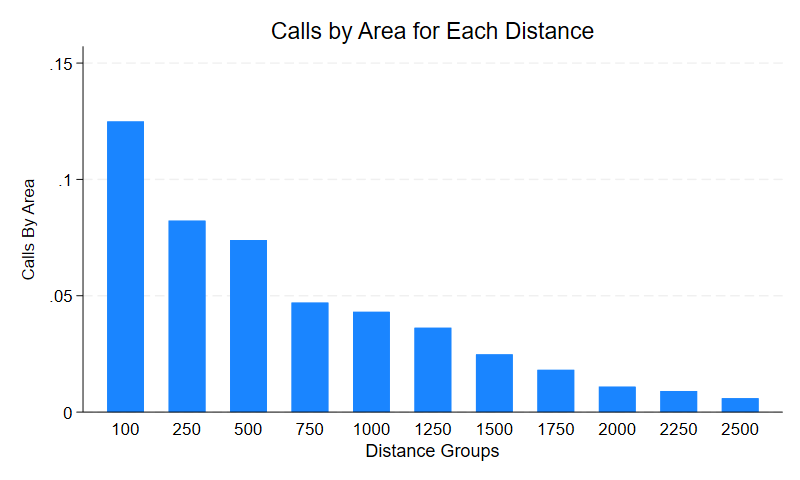
\includegraphics[width=0.5\linewidth]{Reproducibility Package//Visual Graphics/Avg_Calls_per_Distance_Group.png}
    \caption{Enter Caption}
    \label{fig:enter-label}
\end{figure}
\vskip.3in
\begin{abstract}
Here is where I put in information for the abstract
\end{abstract}

\section{Introduction} \label{sec:question}

Our study examines whether drug treatment or rehab centers have a positive or negative correlation with the number of 911 calls in an area. This study itself focuses on the city of Detroit and its metropolitan area. At first, our group thought that the implementation of a drug rehab center in an area would reduce the number of 911 calls. This is caused by a reduction in drug and alcohol misuse; activities that are the main causes of many other illegal activities. In addition to that, drug and alcohol addictions have shown a direct negative correlation with quality of life. For this reason, our initial hypothesis is as follows: How does the distance to the closest drug rehabilitation center relate to the number of calls to 911? To show opposite of our hypothesis, preliminary research further built upon in the literature review shows that prosperous communities prefer not to have drug treatment or rehab centers anywhere near them. This is because these centers have a reputation for affecting people who could be a danger to the community around them. In addition to this, our group hypothesized that the number of 911 calls would decrease with time as the rehab center was in a community for longer. This is because rehab centers are positive aspects of the communities that need them, offering the necessary advice to vulnerable people. The longer a community has a rehab center in it, the more prosperous it would be and the less 911 calls it would need. 

\section{Literature Review}


\section{Data} \label{sec:literature}

Our first dataset consists of 911 call data complied by the Detroit, MI police. This data includes the time and date of the call, the coordinate location of the incident, the zip-code it took place in, as well as the type of crime that was reported. Our second data set is for the drug rehabilitation/mental health treatment center locations. This set includes the addresses of the facilities, the years of operation, and the type of services offered by each treatment center.

\subsection{911 Calls in Detroit Area}
\begin{itemize}
  \item This data comes from the City of Detroit Open Data Portal's Police Serviced 911 Calls  \href{https://data.detroitmi.gov/datasets/detroitmi::police-serviced-911-calls/about}{911 Data}
  \item It is generated by the Detroit Police Department's Crime Data Analytics  when a call is placed
  \item This data set covers 911 calls that are received by precincts around the Detroit metropolitan area from the year 2016-2022
  \item There are 26 variables in this set, the most important for us being Date/Time, Location (Long/Lat), and the zip code that location corresponds to
  \item There are a total of 1.6 million call observations that each have 26 variables however some of the variables are missing data for many of the observations due to certain data points only being recorded if an officer was dispatched.
\end{itemize}

\subsection{Substance Abuse Treatment Centers in Detroit Area}
    \begin{itemize}
        \item This data is from the Substance Abuse and Mental Health Services Administration (SAMHSA) (link not known yet)
  \item Data is generated through the National Survey of Substance Abuse Treatment Services (N-SSATS), an annual survey of all known public and private substance abuse treatment services in the United States. SAMHSA conducts this survey annually.
  \item This data covers the names and addresses of substance abuse treatment services in operation in the Detroit Metropolitan area between the years from 2015-2021. 
  \item There are 55 variables total. There are 333 observations total. 
  \item The most important includes the addresses, latitude and longitude, and year variables. 
  \item   The dataset also includes variables about the centers, including their primary focus, serving setting (in patient, out patient, etc.) and type of care services provided that can be used for further analysis.
  \end{itemize}


\subsection{Data Acquisition}
\label{sec:theory}
How we acquired our datasets:
\begin{itemize}
    \item The 911 calls used in the study between the years of 2016-2022 were from the "City of Detroit Open Data Portal" under the Police Serviced 911 calls section here:
    \url{https://data.detroitmi.gov/datasets/detroitmi::police-serviced-911-calls/about}. Press the download button at the top of the page. Download the "csv" option from the pop up on the left.
    \item The data for the drug treatment centers in and around Wayne County that were used in this study were provided by the Substance Abuse and Mental Health Services Administration  (samhsa) from Dr. Deza. She directly sent us the data, and told us the data originated from SAMHSA. However, we have yet to be able to find exactly how she pulled the data from SAMHSA;
    \url{link not known yet}
\end{itemize}

\noindent Where our data is stored
\begin{itemize}
    \item Most of our data is stored on our GitHub repository our master documentation file has quick links to access each critical piece of data: \href{https://github.com/ecn310/course-project-zipcentercrime/blob/main/Master%20Documentation%20File.md}{Master File}
     \item Any of our files that are too large for GitHub have been stored on a one-drive linked here: \href{https://sumailsyr-my.sharepoint.com/:f:/r/personal/wrmaechl_syr_edu/Documents/ZipCenterCrime?csf=1&web=1&e=IK0GWY}{Drive Access}
\end{itemize}


\subsection{Data Manipulation}
\label{sec:data}

Steps we have taken and plan to take towards data analysis 
\begin{itemize}
    \item  We created a data set from the original calls\_final data hat includes only the observations with missing zip codes, so that we can begin to fill in the missing information
    \begin{itemize}
        \item The link to this data set, "missing\_zip\_code\_calls" can be found in the zipcentercrime repo under code/missing zip codes/access\_to\_missing\_zip\_codes\_data\_set.md or follow this link:  \url{https://sumailsyr-my.sharepoint.com/my?id=%2Fpersonal%2Fregaudre%5Fsyr%5Fedu%2FDocuments%2FECN%20310%20%2D%20Zip%20Center%20Crime%20data} directly to the data because the data set is to large to directly uplaod Github.
        \item The do-file describing how this data set was created can also be found in the zipcentercrime repo under code/missing zip codes/\href{https://github.com/ecn310/course-project-zipcentercrime/blob/main/Missing\%20zip\%20codes/missing_zip_code_create.do}{missing\_zip\_code\_create.do}  
    \end{itemize}
    \item We have also gone through and separated both the 911 call data and the treatment center data by year for future analysis of the data by year
    \begin{itemize}
        \item The 911 call data by year can be found in the zipcentercrime repo under code/Data by year/911 call data by year. The 2016 data is directly uploaded to GitHub while the 2017-2022 data is is linked through .md files because the data sets are too large to directly upload to GitHub.
        \item The do-files used to separate and create the yearly 911 call data sets can also be found in the zipcentercrime repo under code/Data by year/911 call data by year/do files
        \item The treatment center data by year can be found in the zipcentercrime repo under code/Data by year/Treatment center data by year where all the .dta files are directly uploaded to GitHub.
        \item The do-files used to separate and create the yearly Treatment center data can also be found in the zipcentercrime repo under code/Data by year/Treatment center data by year/do files
    \end{itemize}
\item We also intend to drop outlying observations from the calls\_final data set by calculating and dropping any points in the top 1\% of average distance
\item We will look at cross-sectional data, ideally within the years of 2017-2019. We believe that 911 data and/or drug treatment center may be skewed due to COVID-19 impacting the economy and behaviors between 2020-2022. (We need to find article justifying this besides just common sense and anecdotes). 
\item We may look in those time to see if a drug treatment center has opened or closed and the impact it has had on close 911 calls, as well the services of rehab services offered. 
\end{itemize}

\subsection{Linking Datasets}
\label{sec:discussion}

\begin{itemize}
    \item We will merge the 911 calls data to the treatment center data through the location. In the 911 call the location data variables are called \textit{longitude} and \textit{latitude} and the treatment center location data variables are also called \textit{longitude} and \textit{latitude}.
\end{itemize}

\subsection{Notes from 11/14/24:}
\begin{itemize}
    \item think about the opening and closing potentially
    \item Think about how to deal with the farther data points and potentially overlapping, sharing
    \item Only isolate 911 calls to specific drug related ones 
    \item doing zip code level with population density data and number of 911 calls in each density
    \item Only doing this in 2017 - specific we are only analyzing 2017, not just each year
\end{itemize}

\subsection{Key Variables}
\label{sec:result}

\subsection{911 Calls}
\begin{itemize}
    \item Location (longitude/latitude)
    \item Year
    \item If the call was responded to
\end{itemize}

\subsection{Treatment Centers}
\begin{itemize}
    \item Location (Longitude/Latitude)
    \item Primary Service Offered
    \item Year
\end{itemize}

\subsection{Running Analysis}
\label{Data Manipulation and Analysis}
\begin{itemize}
    \item ArcGIS
    \item Stata Analysis
\end{itemize}

\section{Results}

\section{Discussion}

\section{Conclusion}

\section{References}
\end{document}